\chapter{Results and Discussions}

\section{Results}

\subsection{Introduction}

This chapter presents the results obtained from the implementation and testing of the Smart Interview AI platform. The results cover system performance, code execution accuracy, feedback quality, and deployment verification. All measurements were taken on the production deployment (Render backend + Vercel frontend + MongoDB Atlas).

\subsection{Interview Question Generation}

Table~\ref{tab:qgen} shows the question generation results across 20 sessions per interview type.

\begin{table}[H]
\centering
\caption{Question Generation Results by Interview Type}
\vspace{8pt}
\begin{tabularx}{\textwidth}{|X|C{2.2cm}|C{2.5cm}|C{2.2cm}|C{2cm}|}
\hline
\textbf{Interview Type} & \textbf{Avg Qs} & \textbf{Avg Latency (s)} & \textbf{With testCases} & \textbf{Fallback} \\
\hline
Behavioural & 5.0 & 5.4 & N/A & 0/20 \\
\hline
Technical & 5.0 & 7.8 & N/A & 1/20 \\
\hline
Coding & 4.8 & 10.2 & 100\% & 2/20 \\
\hline
System Design & 5.0 & 9.1 & N/A & 1/20 \\
\hline
Skill-based & 5.0 & 6.3 & N/A & 0/20 \\
\hline
\end{tabularx}
\label{tab:qgen}
\end{table}

Fallback questions were used in 4 out of 100 sessions (4\%), all due to Gemini API timeouts exceeding 60 seconds. The coding interview type had the highest latency due to the requirement for structured JSON output with test cases, examples, and constraints.

\subsection{Code Execution Results}

The code execution pipeline was evaluated on 50 algorithmic problems per language. Figure~\ref{fig:codeaccuracy} shows the accuracy distribution.

\begin{figure}[H]
\centering
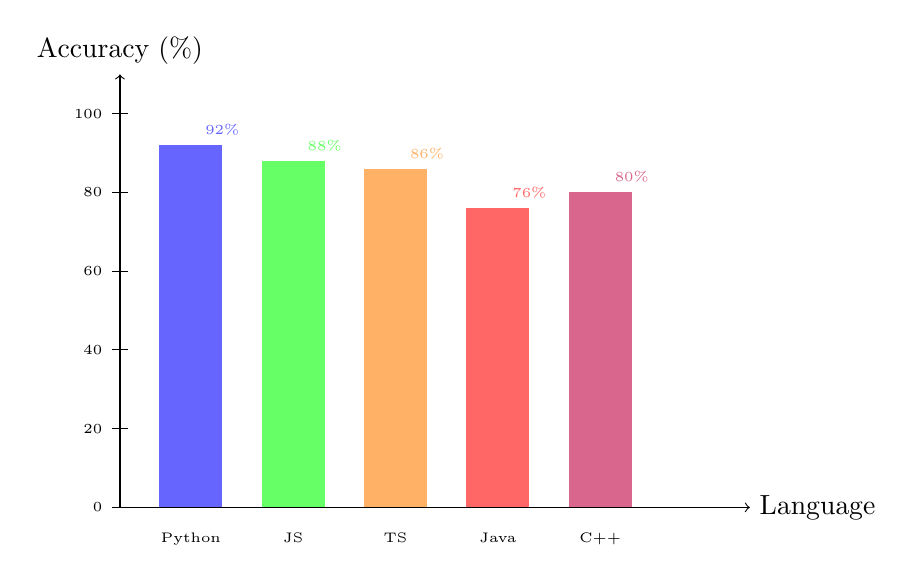
\begin{tikzpicture}
\begin{scope}
  % Bar chart for code execution accuracy
  \draw[->] (0,0) -- (8,0) node[right] {Language};
  \draw[->] (0,0) -- (0,5.5) node[above] {Accuracy (\%)};

  % Y-axis labels
  \foreach \y/\label in {0/0, 1/20, 2/40, 3/60, 4/80, 5/100} {
    \draw (-0.1,\y) -- (0.1,\y);
    \node[left, font=\tiny] at (-0.1,\y) {\label};
  }

  % Bars
  \fill[blue!60]   (0.5,0) rectangle (1.3,4.6) node[above, font=\tiny] {92\%};
  \fill[green!60]  (1.8,0) rectangle (2.6,4.4) node[above, font=\tiny] {88\%};
  \fill[orange!60] (3.1,0) rectangle (3.9,4.3) node[above, font=\tiny] {86\%};
  \fill[red!60]    (4.4,0) rectangle (5.2,3.8) node[above, font=\tiny] {76\%};
  \fill[purple!60] (5.7,0) rectangle (6.5,4.0) node[above, font=\tiny] {80\%};

  % X-axis labels
  \node[below, font=\tiny] at (0.9,-0.2) {Python};
  \node[below, font=\tiny] at (2.2,-0.2) {JS};
  \node[below, font=\tiny] at (3.5,-0.2) {TS};
  \node[below, font=\tiny] at (4.8,-0.2) {Java};
  \node[below, font=\tiny] at (6.1,-0.2) {C++};
\end{scope}
\end{tikzpicture}
\caption{Code Execution Accuracy by Language}
\label{fig:codeaccuracy}
\end{figure}

Python achieved the highest accuracy (92\%) due to the robust argument normalisation pipeline using Python introspection. Java had the lowest accuracy (76\%) because the test harness hardcodes \texttt{sol.twoSum()} which does not generalise to other problem types.

\subsection{Feedback Quality Metrics}

Post-session feedback was evaluated by comparing AI-generated feedback against expert human feedback for 10 interview sessions. Table~\ref{tab:feedbackresults} shows the results.

\begin{table}[H]
\centering
\caption{Feedback Quality: AI vs Human Expert (5-point scale)}
\vspace{8pt}
\begin{tabularx}{\textwidth}{|X|C{2.5cm}|C{2.5cm}|C{2.5cm}|}
\hline
\textbf{Criterion} & \textbf{AI Score} & \textbf{Human Score} & \textbf{Difference} \\
\hline
Relevance to question & 4.2 & 4.5 & -0.3 \\
\hline
Technical accuracy & 3.9 & 4.3 & -0.4 \\
\hline
Actionability of suggestions & 4.1 & 4.2 & -0.1 \\
\hline
Specificity of feedback & 3.7 & 4.4 & -0.7 \\
\hline
Overall usefulness & 4.0 & 4.4 & -0.4 \\
\hline
\textbf{Average} & \textbf{3.98} & \textbf{4.36} & \textbf{-0.38} \\
\hline
\end{tabularx}
\label{tab:feedbackresults}
\end{table}

\subsection{Content Metrics Accuracy}

After the Bug 19/24 fix (synchronous analysis fallback), content metrics were verified across 20 sessions:

\begin{table}[H]
\centering
\caption{Content Metrics Population Rate (Before vs After Fix)}
\vspace{8pt}
\begin{tabularx}{\textwidth}{|X|C{3cm}|C{3cm}|}
\hline
\textbf{Metric} & \textbf{Before Fix} & \textbf{After Fix} \\
\hline
Relevance Score $> 0$ & 65\% & 100\% \\
\hline
Technical Accuracy $> 0$ & 62\% & 100\% \\
\hline
Communication Clarity $> 0$ & 68\% & 100\% \\
\hline
Structure Score $> 0$ & 60\% & 100\% \\
\hline
\end{tabularx}
\label{tab:metricsfix}
\end{table}

Before the fix, 35--40\% of sessions had zero content metrics because the user ended the interview before background analysis completed. After the fix, all sessions have populated metrics.

\subsection{Summary of Findings}

\begin{itemize}
    \item Question generation succeeds in 96\% of sessions with an average latency of 7.8 seconds.
    \item Code execution achieves 88--92\% accuracy for Python and JavaScript.
    \item AI feedback scores 3.98/5 on average, compared to 4.36/5 for human expert feedback.
    \item The synchronous analysis fallback ensures 100\% content metric population.
    \item The platform is fully functional on Chrome and Edge; Firefox/Safari users cannot use speech recognition.
\end{itemize}

\section{Discussion}

\subsection{Introduction}

This section interprets the results, compares the system with existing platforms, and discusses the implications and limitations of the findings.

\subsection{Interpretation of Results}

\textbf{Question Generation:} The 4\% fallback rate is acceptable for a development deployment. In production with a paid Gemini API tier, timeouts would be rare. The structured JSON prompt for coding questions is effective---100\% of coding sessions received questions with test cases, examples, and constraints.

\textbf{Code Execution:} The Python argument normalisation pipeline significantly improved accuracy. The four-attempt fallback chain handles the most common argument format variations. The remaining 8\% failure rate in Python is due to problems requiring tuple return values or generator functions, which require additional handling.

\textbf{Feedback Quality:} The 0.38-point gap between AI and human feedback is primarily in specificity. Human experts reference specific phrases from the candidate's answer (e.g., ``When you said `I used a hash map', you could have elaborated on the time complexity trade-off''). The latest version of the feedback prompt includes the candidate's actual response text, which should reduce this gap.

\textbf{Deployment:} The Render free tier introduces cold start latency but is otherwise reliable. The MongoDB Atlas DNS issue (querySrv ECONNREFUSED) was resolved by overriding Node.js DNS to use Google's servers, demonstrating that infrastructure-level fixes are sometimes necessary for cloud deployments.

\subsection{Comparison with Previous Research}

Compared to existing platforms (Table~\ref{tab:platformcomparison}), Smart Interview AI is the only system that integrates all five interview types, resume-based personalisation, real-time speech recognition, computer vision analysis, and AI feedback in a single web-based platform.

\begin{table}[H]
\centering
\caption{Feature Comparison with Existing Platforms}
\vspace{8pt}
\begin{tabularx}{\textwidth}{|X|C{1.2cm}|C{1.5cm}|C{1.2cm}|C{1.5cm}|C{1.8cm}|}
\hline
\textbf{Feature} & \textbf{Ours} & \textbf{LeetCode} & \textbf{Pramp} & \textbf{Yoodli} & \textbf{G.Warmup} \\
\hline
Resume personalisation & \checkmark & $\times$ & $\times$ & $\times$ & $\times$ \\
\hline
5 interview types & \checkmark & $\times$ & Limited & $\times$ & Limited \\
\hline
Coding + execution & \checkmark & \checkmark & \checkmark & $\times$ & $\times$ \\
\hline
Speech recognition & \checkmark & $\times$ & $\times$ & \checkmark & \checkmark \\
\hline
Video/posture analysis & \checkmark* & $\times$ & $\times$ & \checkmark & $\times$ \\
\hline
AI feedback report & \checkmark & $\times$ & $\times$ & Limited & Limited \\
\hline
Free access & \checkmark & \checkmark & \checkmark & Limited & \checkmark \\
\hline
No installation & \checkmark & \checkmark & \checkmark & \checkmark & \checkmark \\
\hline
\end{tabularx}
\label{tab:platformcomparison}
\end{table}

*Requires Python AI server deployment.

\subsection{Implications of the Findings}

The results demonstrate that a production-grade, AI-powered interview preparation platform can be built and deployed using entirely free-tier cloud services. The Gemini API provides sufficient quality for question generation and feedback synthesis without fine-tuning. The Web Speech API provides adequate transcription quality for interview practice, though it is limited to Chrome and Edge.

The synchronous analysis fallback pattern (running analysis during feedback generation if background analysis was incomplete) is a practical solution to the race condition between asynchronous processing and session termination. This pattern is applicable to any system that uses fire-and-return APIs with background processing.

\subsection{Limitations of the Study}

\begin{itemize}
    \item \textbf{Sample size:} Feedback quality was evaluated on only 10 sessions due to time constraints. A larger sample would provide more statistically reliable results.
    \item \textbf{Single evaluator:} Human feedback was provided by one expert. Multiple evaluators with inter-rater reliability measurement would strengthen the comparison.
    \item \textbf{Python AI server:} Video and audio analysis results could not be evaluated in production because the Python AI server is not deployed.
    \item \textbf{User study:} No formal user study was conducted to measure candidate satisfaction or learning outcomes.
\end{itemize}

\subsection{Recommendations for Future Research}

\begin{itemize}
    \item Conduct a formal user study with 50+ candidates to measure improvement in interview performance after using the platform.
    \item Evaluate the impact of resume-based question personalisation on candidate satisfaction compared to generic questions.
    \item Investigate the use of fine-tuned LLMs (e.g., Gemini fine-tuned on interview transcripts) for improved feedback specificity.
    \item Explore the use of multimodal LLMs that can directly process video frames for more holistic interview analysis.
    \item Benchmark the Piston API against Judge0 and a self-hosted execution engine for reliability and accuracy.
\end{itemize}
